% This file is part of the stream_information project.
% Copyright 2017 the authors. All rights reserved.

% TODO:
% - Reference for the dustmaps package? See software section.

% Story:
% - progenitor - show std_v, std_phi2
% - 2 gaps, 1 under-density - epicycles/streakline? percentiles in polynomial
% - spur - encounter?

\documentclass[modern]{aastex62}

\usepackage{amsmath}

% typography
\setlength{\parindent}{1.\baselineskip}
\newcommand{\acronym}[1]{{\small{#1}}}
\newcommand{\package}[1]{\textsl{#1}}
\newcommand{\gaia}{\textsl{Gaia}}
\newcommand{\pans}{\textsl{Pan-STARRS}}
\newcommand{\DR}{\acronym{DR2}}
\newcommand{\msun}{\textrm{M}_\odot}
\newcommand{\kpc}{\textrm{kpc}}
% \newcommand{\mag}{\textrm{mag}}
\newcommand{\kms}{\ensuremath{\textrm{km}~\textrm{s}^{-1}}}
\newcommand{\bs}[1]{\boldsymbol{#1}}
\newcommand{\masyr}{\ensuremath{\textrm{mas}~\textrm{yr}^{-1}}}
\newcommand{\feh}{\ensuremath{[\textrm{Fe} / \textrm{H}]}}
\newcommand{\article}{\textsl{Letter}}

\newcommand{\sectionname}{Section}
\newcommand{\equationname}{Equation}
\renewcommand{\tablename}{Table}

\newcommand{\todo}[1]{{\color{red} TODO: #1}}

% aastex parameters
% \received{not yet; THIS IS A DRAFT}
%\revised{not yet}
%\accepted{not yet}
% % Adds "Submitted to " the arguement.
% \submitjournal{ApJ}
\shorttitle{GD-1 in Gaia DR2}
\shortauthors{Price-Whelan \& Bonaca}

%@arxiver{}

\begin{document}\sloppy\sloppypar\raggedbottom\frenchspacing % trust me

\title{Off the beaten path: \\
       Gaia reveals GD-1 stars perturbed off of the main stream track}
% Gaia DR2 reveals stream stars...
% A first look at the GD-1 stellar stream with Gaia DR2

\author[0000-0003-0872-7098]{Adrian~M.~Price-Whelan}
\altaffiliation{These authors contributed equally to this work.}
\affiliation{Department of Astrophysical Sciences,
             Princeton University, Princeton, NJ 08544, USA}
\email{adrn@astro.princeton.edu}
\correspondingauthor{Adrian M. Price-Whelan}

\author[0000-0002-7846-9787]{Ana Bonaca}
\altaffiliation{These authors contributed equally to this work.}
\affil{Harvard--Smithsonian Center for Astrophysics, Cambridge, MA 02138, USA}

\begin{abstract}\noindent % trust me
Tidally-disrupted globular clusters are transformed into thin, dynamically-cold
streams of stars that are extremely valuable tracers of the large- and
small-scale distribution of mass in the Galaxy.
Most stellar streams discovered around the Milky Way reside in the Galactic halo
and are therefore primarily sensitive to the dark matter distribution.
We present a sample of highly-probable members of the longest cold stream, GD-1,
selected to have small parallaxes and retrograde proper motions using data from
the \gaia\ mission, and \pans\ photometry consistent with an old and metal-poor
population at a distance of $\sim10~\kpc$.
This selection extended the stream by $20^\circ$, revealed a possible location of the progenitor and mapped significant density variations along the stream in unprecedented detail.
In addition to several prominent gaps, for the first time we also find evidence of stream members off the main track.
No(?) secular formation mechanisms predict the existence of such spurs, but they are a natural result of a stream interaction with a massive perturber.
Using the impulse approximation arguments, we estimate that the detected underdensity and the associated spur could have been induced by a perturbation of a $\sim10^7\,\rm M_\odot$(?) object $\sim 0.5\,$Gyr ago.
Our model of GD-1 indicates that the stream crosses the Galactic plane at a large radius, which puts the likely origin of the perturber beyond the stellar disk.
\end{abstract}

\keywords{Galaxy: halo --- dark matter}

\section{Introduction}
\label{sec:intro}

Dynamically cold stellar streams are formed from the tidal disruption of stellar
systems by the gravitational field of their host galaxy.
The phase-space density and mean track of stars in streams therefore encode
information about the underlying distribution and shape of mass on galactic
scales (e.g., \citealt{Johnston:1999, Bonaca:2018}).
Most stellar streams are found in the halos of galaxies and are therefore
important tracers of the large-scale distribution of dark matter in galactic
halos.

Long, thin stellar streams are also excellent laboratories for studying
small-scale structures in the mass distribution:
thin streams can remain coherent for tens of orbital periods, depending in
detail on the symmetries of the underlying galactic mass distribution (e.g.,
\citealt{Erkal:2016a}).
Encounters between massive perturbers and stream stars imprint variations in the
phase-space density that can persist and remain visible for close to their total
survival time (e.g., \citealt{Yoon:2011}).
In this sense, streams represent one of the most promising directions for
testing the existence of small-scale dark matter sub-halos, predicted by
standard $\Lambda$ Cold Dark Matter ($\Lambda$CDM) theory
(\citealt{Erkal:2015, Sanders:2016, Bovy:2017}).

Over 30 candidate stellar streams have been discovered throughout the halo of
the Milky Way, thanks to large-area, multi-band photometric surveys (especially
the Sloan Digital Sky Survey, SDSS; \citealt{York:2000}).
The Milky Way streams have a wide range of properties such as length, velocity
dispersion, and density (e.g., \citealt{Odenkirchen:2001, Grillmair:2006,
Grillmair:2006b, Belokurov:2006, Belokurov:2007, Bonaca:2012, Shipp:2018}; see
also the recent review \citealt{Grillmair:2016, Newberg:2016}), and the majority
have no obvious, bound progenitor systems;
of the thin, likely globular-cluster-origin streams, only two have clear
progenitors (NGC 5466 and Palomar 5).

The most prominent and longest (in angular extent) thin stream is the GD-1
stream (named after its discoverers; \citealt{Grillmair:2006}).
GD-1 was found using a matched filter on photometric data from the SDSS and
was found to span $\approx 60^\circ$ in Heliocentric sky coordinates, partially
because of its relative proximity to the Sun ($\approx 7$--$10~\textrm{kpc}$).
Despite being close and relatively high surface-density, no remnant progenitor
cluster or stellar system has been found associated with the stream, but its
width,  metallicity ($\feh \approx -1.4$; \citealt{Koposov:2010}) and estimated
stellar mass ($M \approx 2 \times 10^4~\msun$; \citealt{Koposov:2010}) are
consistent with being a disrupted globular cluster.

The long physical length of the GD-1 stream ($\sim 15~\kpc$) and location in the
Galactic halo (pericentric distance $r_\textrm{peri} \sim 13~\kpc$) make it an
ideal object for constraining the gravitational potential of dark matter in the
inner Milky Way.
Indeed, both from fitting orbits to binned phase-space measurements along the
GD-1 stream (\citealt{Koposov:2010}) and from modeling the stream track in
phase-space coordinates \citep{Bowden:2015, Bovy:2016}, it has been used to show that the
dark matter distribution within its orbit is consistent with being close to
spherical.

Its long length --- and therefore its implied old dynamical age --- combined
with its particular orbit also make it a prime stream to search for interactions
with dark matter subhalos:
because of its large pericentric distance and retrograde orbit with respect to
the Galactic bar, density variations in the stream are not expected from either
interactions with giant molecular clouds (\citealt{Amorisco:2016}) or resonant
encounters with the bar (\citealt{Pearson:2017}).
By estimating a stream age of $\approx 4~\textrm{Gyr}$ assuming a progenitor
mass of $10^5~\msun$, and by taking a subhalo mass function and density from
XXX, \citet{Erkal:2016} predict that GD-1 could have up to one significant, wide
($\approx 5$--$7^\circ$) gap caused by an interaction with a
$10^6$--$10^7~\msun$ subhalo.
\todo{implications of subhalo detection (cite bullock review along the lines: on small scales, lcdm has some issues, so alternative classes of models proposed, some that lack structure on small scales; so ruling on the existence of subhalos expected to be detectable with GD-1 directly informs the nature of dark matter.)}

\todo{hints of density variations} from initial work Koposov:2010, later confirmed by density modeling, but all low significance
(\citealt{Carlberg:2013}).
More recently, deep photometry of GD-1 from CFHT/Megacam has revealed
interesting small-scale ``wiggles'' and significant density variations along a $\approx 45^\circ$ span of the stream (\citealt{DeBoer:2018}):
[summarize their conclusions].
\todo{these analyses relied on binned data, still contaminated by MW stars}

In this \article, we present clearest view of the GD-1 stream to date using
astrometric data from the \gaia\ mission data release 2 (\DR) combined with
precise photometry from the \pans\ survey.
We find XX under-densities gaps, some consistent with ...
We revisit...do not try to model or fit for Galactic potential.
Focus on stream properties, data.


\section{Data}
\label{sec:data}

We use astrometric data from the \gaia\ mission (\citealt{Prusti:2016}), data
release 2 (\citealt{Gaia-Collaboration:2018, Lindegren:2018}), and photometry
from the \pans\ survey, data release 1 (\citealt{Chambers:2016}) to select
high-confidence members of the GD-1 stream.

We retrieve \gaia\ data along the previously-identified track of the GD-1 stream
from the \gaia\ science archive\footnote{\url{https://gea.esac.esa.int/}} by
selecting all sources with small parallax, $\varpi < 1~\textrm{mas}$, and use a
set of spherical polygons to select batches of stars that have small latitude in
the heliocentric GD-1 coordinate system, $(\phi_1, \phi_2)$, defined in
\cite{Koposov:2010}.\footnote{This transformation is implemented using the
\package{Astropy} (\citealt{astropy}) coordinate transformation framework in the
\package{Gala} \texttt{Python} package (\citealt{gala}).}
We convert the sky coordinates and proper motions of the parallax-selected stars
to the GD-1 stream coordinate system, and correct the proper motions for solar
reflex motion by assuming that stars at a given stream longitude, $\phi_1$, have
a distance given by the linear relationship $d(\phi_1) = (0.05 \, \phi_1 +
10)~\textrm{kpc}$.
For the solar velocity in a Galactocentric rest frame, we use $\bs{v}_\odot =
(11.1, 232.24, 7.25)~\kms$ (\citealt{Schonrich:2010, Bovy:2015}).
\figurename~\ref{fig:selection} (top right) shows the distribution of stars with
$|\phi_2| < XX^\circ$ in solar-reflex-corrected proper motion components in the
GD-1 coordinate system, $\mu_{\phi_1, \odot}$ (which includes the $\cos{\phi_2}$
term) and $\mu_{\phi_2, \odot}$.
GD-1 member stars are visible as the over-density around
$(\mu_{\phi_1, \odot}, \mu_{\phi_2, \odot}) \approx (-8, 0)~\masyr$.

As a first selection of GD-1 candidate member stars, we select stars with proper
motions $XX < \mu_{\phi_1, \odot} < XX~\masyr$ and $XX < \mu_{\phi_2, \odot} <
XX~\masyr$, as visualized by the rectangle in the top right panel of
\figurename~\ref{fig:selection}.
\figurename~\ref{fig:selection} (top left) shows all stars the pass the
selection on proper motion, plotted in the GD-1 coordinate system.
From kinematic selection alone, the stream is identifiable as the over-density
of stars around $\phi_2 = 0$ between longitudes $XX^\circ \lesssim \phi_1
\lesssim XX^\circ$.

\begin{figure}[h]
\begin{center}
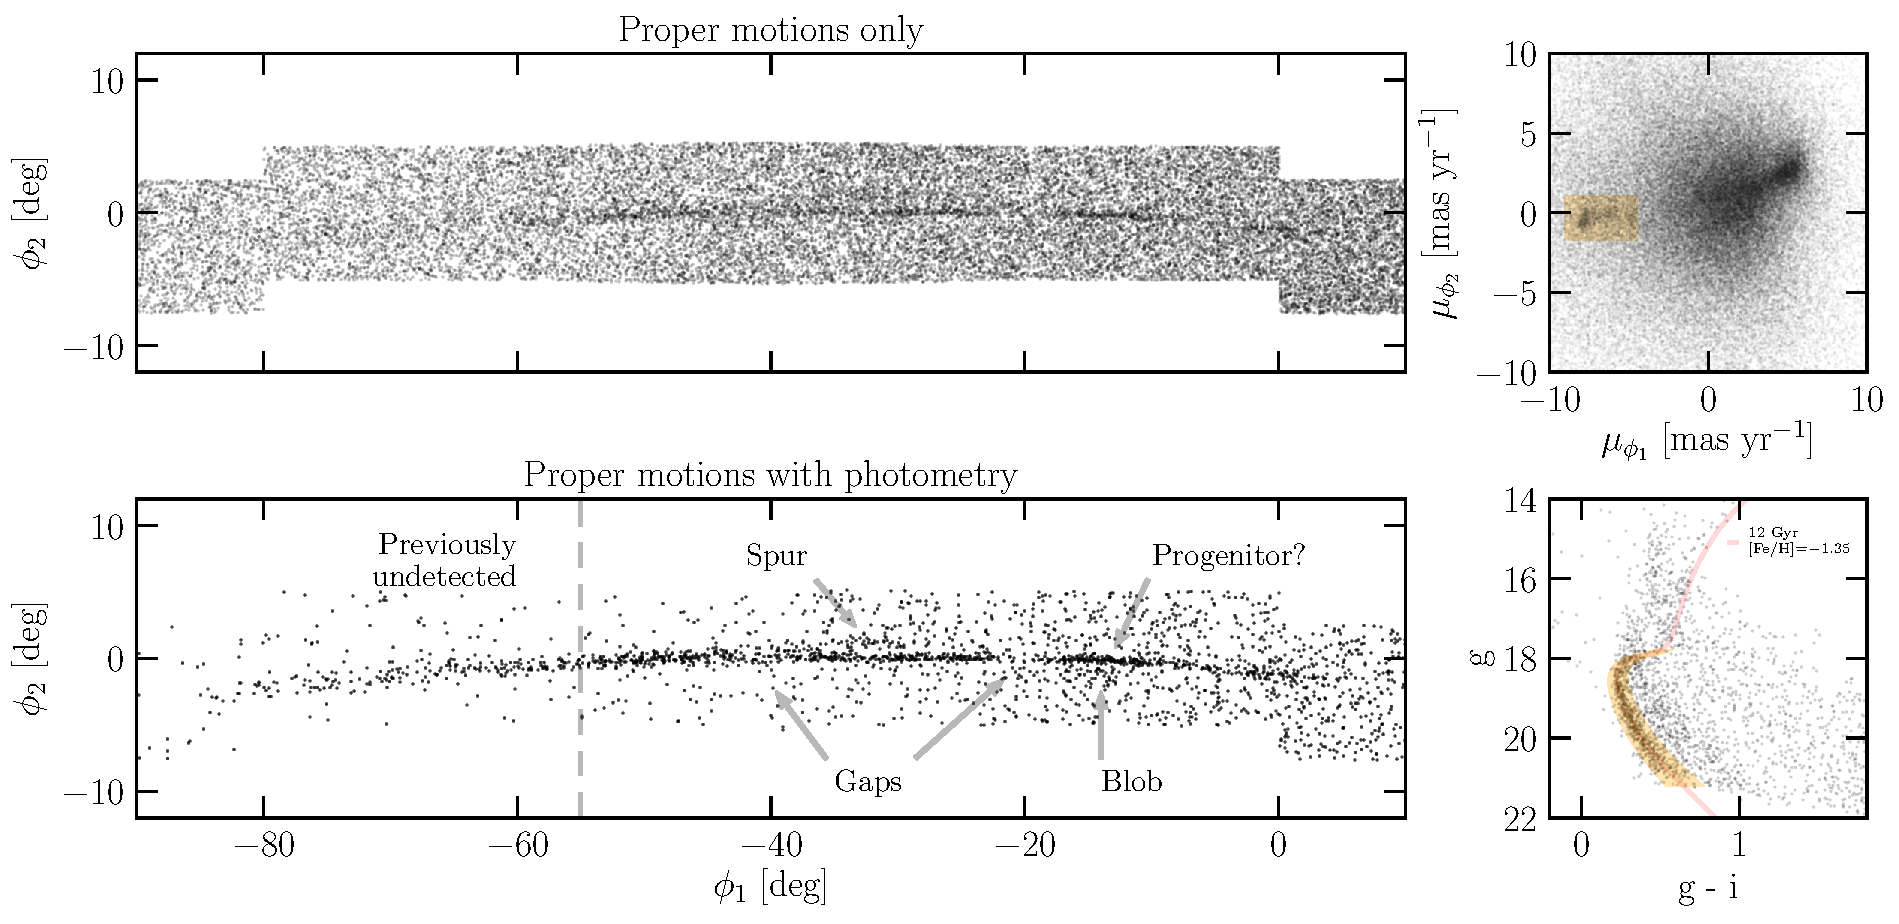
\includegraphics[width=\textwidth]{gd1_sample.pdf}
\end{center}
\caption{
    \todo{AB}
\label{fig:selection}
}
\end{figure}

To improve the contrast of the stream over the background, we cross-match the
sample to the \pans\ photometric catalog and use the photometry to further clean
the sample.
\figurename~\ref{fig:selection} (bottom right) shows the distribution of
proper-motion-selected candidate stream stars in a de-reddened \pans\
color-magnitude diagram (CMD).
\todo{AB: Did you also cut on $phi_2$?}.
The over-plotted isochrone (red line) is from the MESA Isochrones \& Stellar
Tracks (MIST; \citealt{Dotter:2016, Choi:2016, Paxton:2011}) and represents a
$12~\textrm{Gyr}$ old population with $\feh = -1.XX$ at a distance of $XX~\kpc$.
We use this isochrone to motivate a polygonal selection in de-reddened $g-i$
color and apparent $g$-band magnitude, as visualized by the shaded region in the
bottom right panel of \figurename~\ref{fig:selection}.

\figurename~\ref{fig:selection} (bottom left) shows the final sample of GD-1
stream member candidates after selecting on both proper motion and photometry.
The GD-1 stream is clearly visible in the point density of individual stars (the
positions are not binned); this is the most pure view of the stream to date.
The increased contrast shows that the stream extends at least another $20^\circ$
to negative longitudes.
Several of the under-densities and gaps hinted at from photometric selection
alone (\citealt{Koposov:2010, Carlberg:2013}) appear as striking features in
this significantly cleaner density map of the GD-1 stream.
Finally, at least two new features are visible in this new view of the stream:
(1) ``the spur,'' stars above the main stream track (in $\phi_2$) between
$-40^\circ \lesssim \phi_1 \lesssim -30^\circ$, and (2) ``the blob,'' stars
below the main stream track between $-20^\circ \lesssim \phi_1 \lesssim
-10^\circ$.
We discuss each of these in more detail in \sectionname
s~\ref{sec:results}--\ref{sec:discussion} below.


\section{Results}
\label{sec:results}

We extract high-confidence stream stars from the proper motion and CMD selected
sample by further selecting stars close to the main stream track.
We use these main stream track stars to study the global properties of the
stream, and find interesting substructures off of the main stream track.

\subsection{Global properties}
\label{sec:res_global}

To study of global properties of the stream as a function of stream longitude,
we extract stream stars around a low-order polynomial model for the median
stream latitude, $\phi_2$, as a function of stream longitude, $\phi_1$.
In detail, we find stream ridge points by computing a running median in $\phi_2$
in steps of $XX^\circ$ along $\phi_1$, then fit a second-order polynomial to the
ridge points to find $\phi_{2, \textrm{track}}(\phi_1)$.
We define the stream as the region within $\left| \phi_2 - \phi_{2,
\textrm{track}}(\phi_1) \right| < 0.6^\circ$.
\figurename~\ref{fig:XX} (XX panel) again shows the high-confidence
stream stars, and the two curved lines (blue) show the upper and lower boundary
of the stream region.

\begin{figure}[h]
\begin{center}
% \includegraphics[width=\textwidth]{???.pdf}
\end{center}
\caption{%
\todo{???}
\label{fig:XX}
}
\end{figure}

The clearly identifiable portions of the GD-1 stream are located at high
Galactic latitudes ($b > 20^\circ$), and we therefore do not expect significant
dust extinction or variations in extinction within the stream region.
\figurename~\ref{fig:XX} (XX panel) shows the $V$-band extinction
in the region around the GD-1 stream, computed from the
Schlegel-Finkbeiner-Davis extinction map (\cite{Schlegel:1998}; hereafter SFD).
For stream longitudes $-60^\circ < \phi_1 < 10^\circ$ and $-1^\circ < \phi_2 <
1^\circ$, the median $V$-band extinction is $\textrm{med}\left(A_V\right) =
0.04~\textrm{mag}$, and the dispersion in $A_V$ in this region is $\sigma_{A_V}
\approx 0.03~\textrm{mag}$.
For longitudes $\phi_1 < -60^\circ$, as the stream approaches the Galactic disk,
dust extinction becomes more appreciable, and the stream stars are harder to
select apart from the background.

We extract properties of the stream from the stream region defined above as a
function of $\phi_1$ by computing properties in overlapping windows:
we set the window size to $XX^\circ$ in $\phi_1$, and shift the window center by
$1^\circ$ along the stream region.
\figurename~\ref{fig:track-and-model} shows the median latitude, $\phi_2$,
stream surface density, $XX$, stream width, $XX$, and median proper motions,
$\mu_{\phi_1}$ and $\mu_{\phi_2}$, extracted in this way.
For the surface density, we subtract an estimate of the background surface
density by \todo{AB}.
To estimate the stream width, $w$, we compute the median absolute deviation,
$\textrm{MAD}$, and use this to estimate a robust standard deviation, $w = 1.5
\times \textrm{MAD}$.

\todo{Comment on density variations, stream width variations. Do we want a
$\Delta \phi_2$ plot (relative to mean stream track) with 15th/85th
percentiles?}

- first measure density variations in background subtracted profile
- find maximum -- morphology as expected from a progenitor in the final stages of dissolution (cit)
- several prominent gaps: density contrast, width
- some (all?) seen in earlier data
- but not related to dust

We compare the measured stream properties to a simple model for the phase-space
density of the stream, generated by only simulating the orbital evolution of
cluster stars once they are tidally stripped from the progenitor.
In detail, during simulation, star particles are released from the Lagrange
points of the cluster with a spread in position and velocity set by the mass of
the satellite and the location within the host galaxy, with some tunable scale
parameters.
We use the parametrization and adopted scale parameters of \citet{Fardal:2015},
who fit the release distribution parameters by comparing to full $N$-body
simulations across a range of mass and orbital parameters.
This method can accurately reproduce the mean track of the resulting stream, but
the density of stars along the stream depends strongly on the mass-loss history
and internal kinematics of the progenitor system.
Here we assume a constant mass-loss rate, and release stream particles uniformly
in time from each Lagrange point.

To compute initial conditions for the stream model, we fit an orbit to the
observed properties of the stream in a fixed model for the gravitational
potential of the Milky Way.
We use a three-component potential model to represent the Galaxy, consisting of
a Miyamoto-Nagai disk (\citealt{Miyamoto:1975}), a Hernqust bulge
(\citealt{Hernquist:1990}), and a spherical Navarro-Frenk-White dark matter halo
(\citealt{Navarro:1996}).
We set the disk scale-length parameters to closely match the disk model found in
\citet{Bovy:2015}, and other parameters are set to reproduce an approximately
flat rotation curve between $5 < R < 15~\kpc$ with a circular velocity at the
solar circle, $v_{\textrm{circ}, \odot} \approx 230~\kms$.

To initialize the model stream generation, we \todo{...}

Stream properties computed from resulting model stream are plotted in \figurename~\ref{fig:track-and-model} as \todo{XX}.

\begin{figure}[h]
\begin{center}
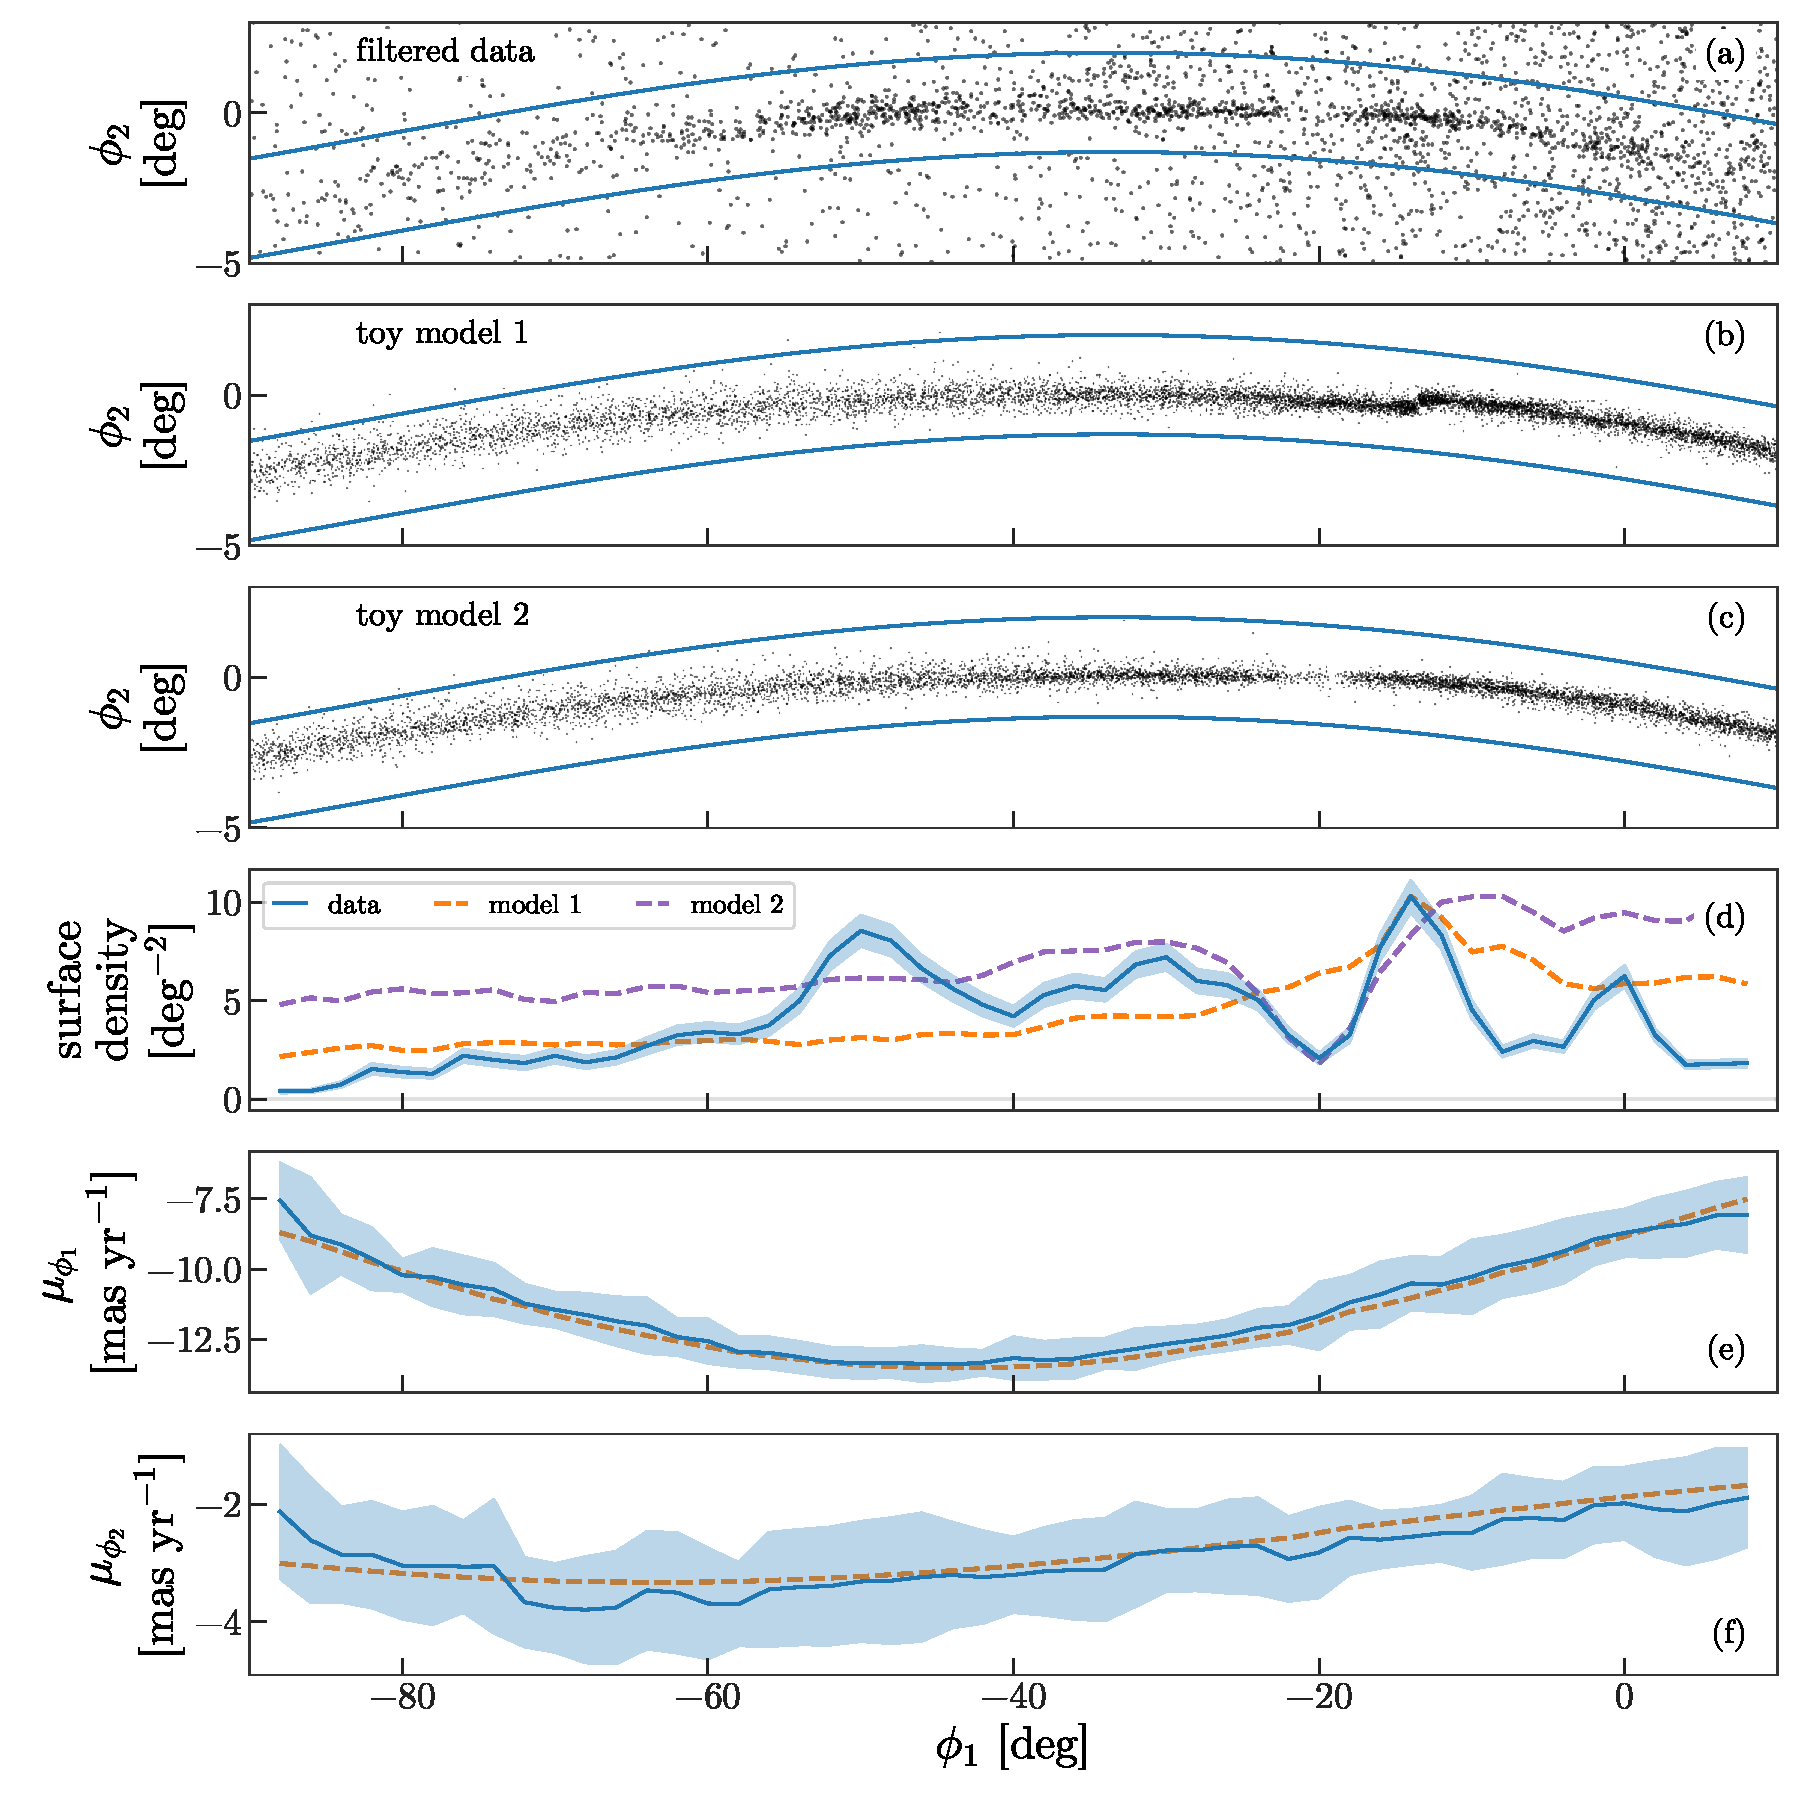
\includegraphics[width=\textwidth]{track_observables.pdf}
\end{center}
\caption{%
\todo{APW}
\label{fig:track-and-model}
}
\end{figure}


\subsection{Off-track features}
\label{sec:res_gap}

\begin{figure}[h]
\begin{center}
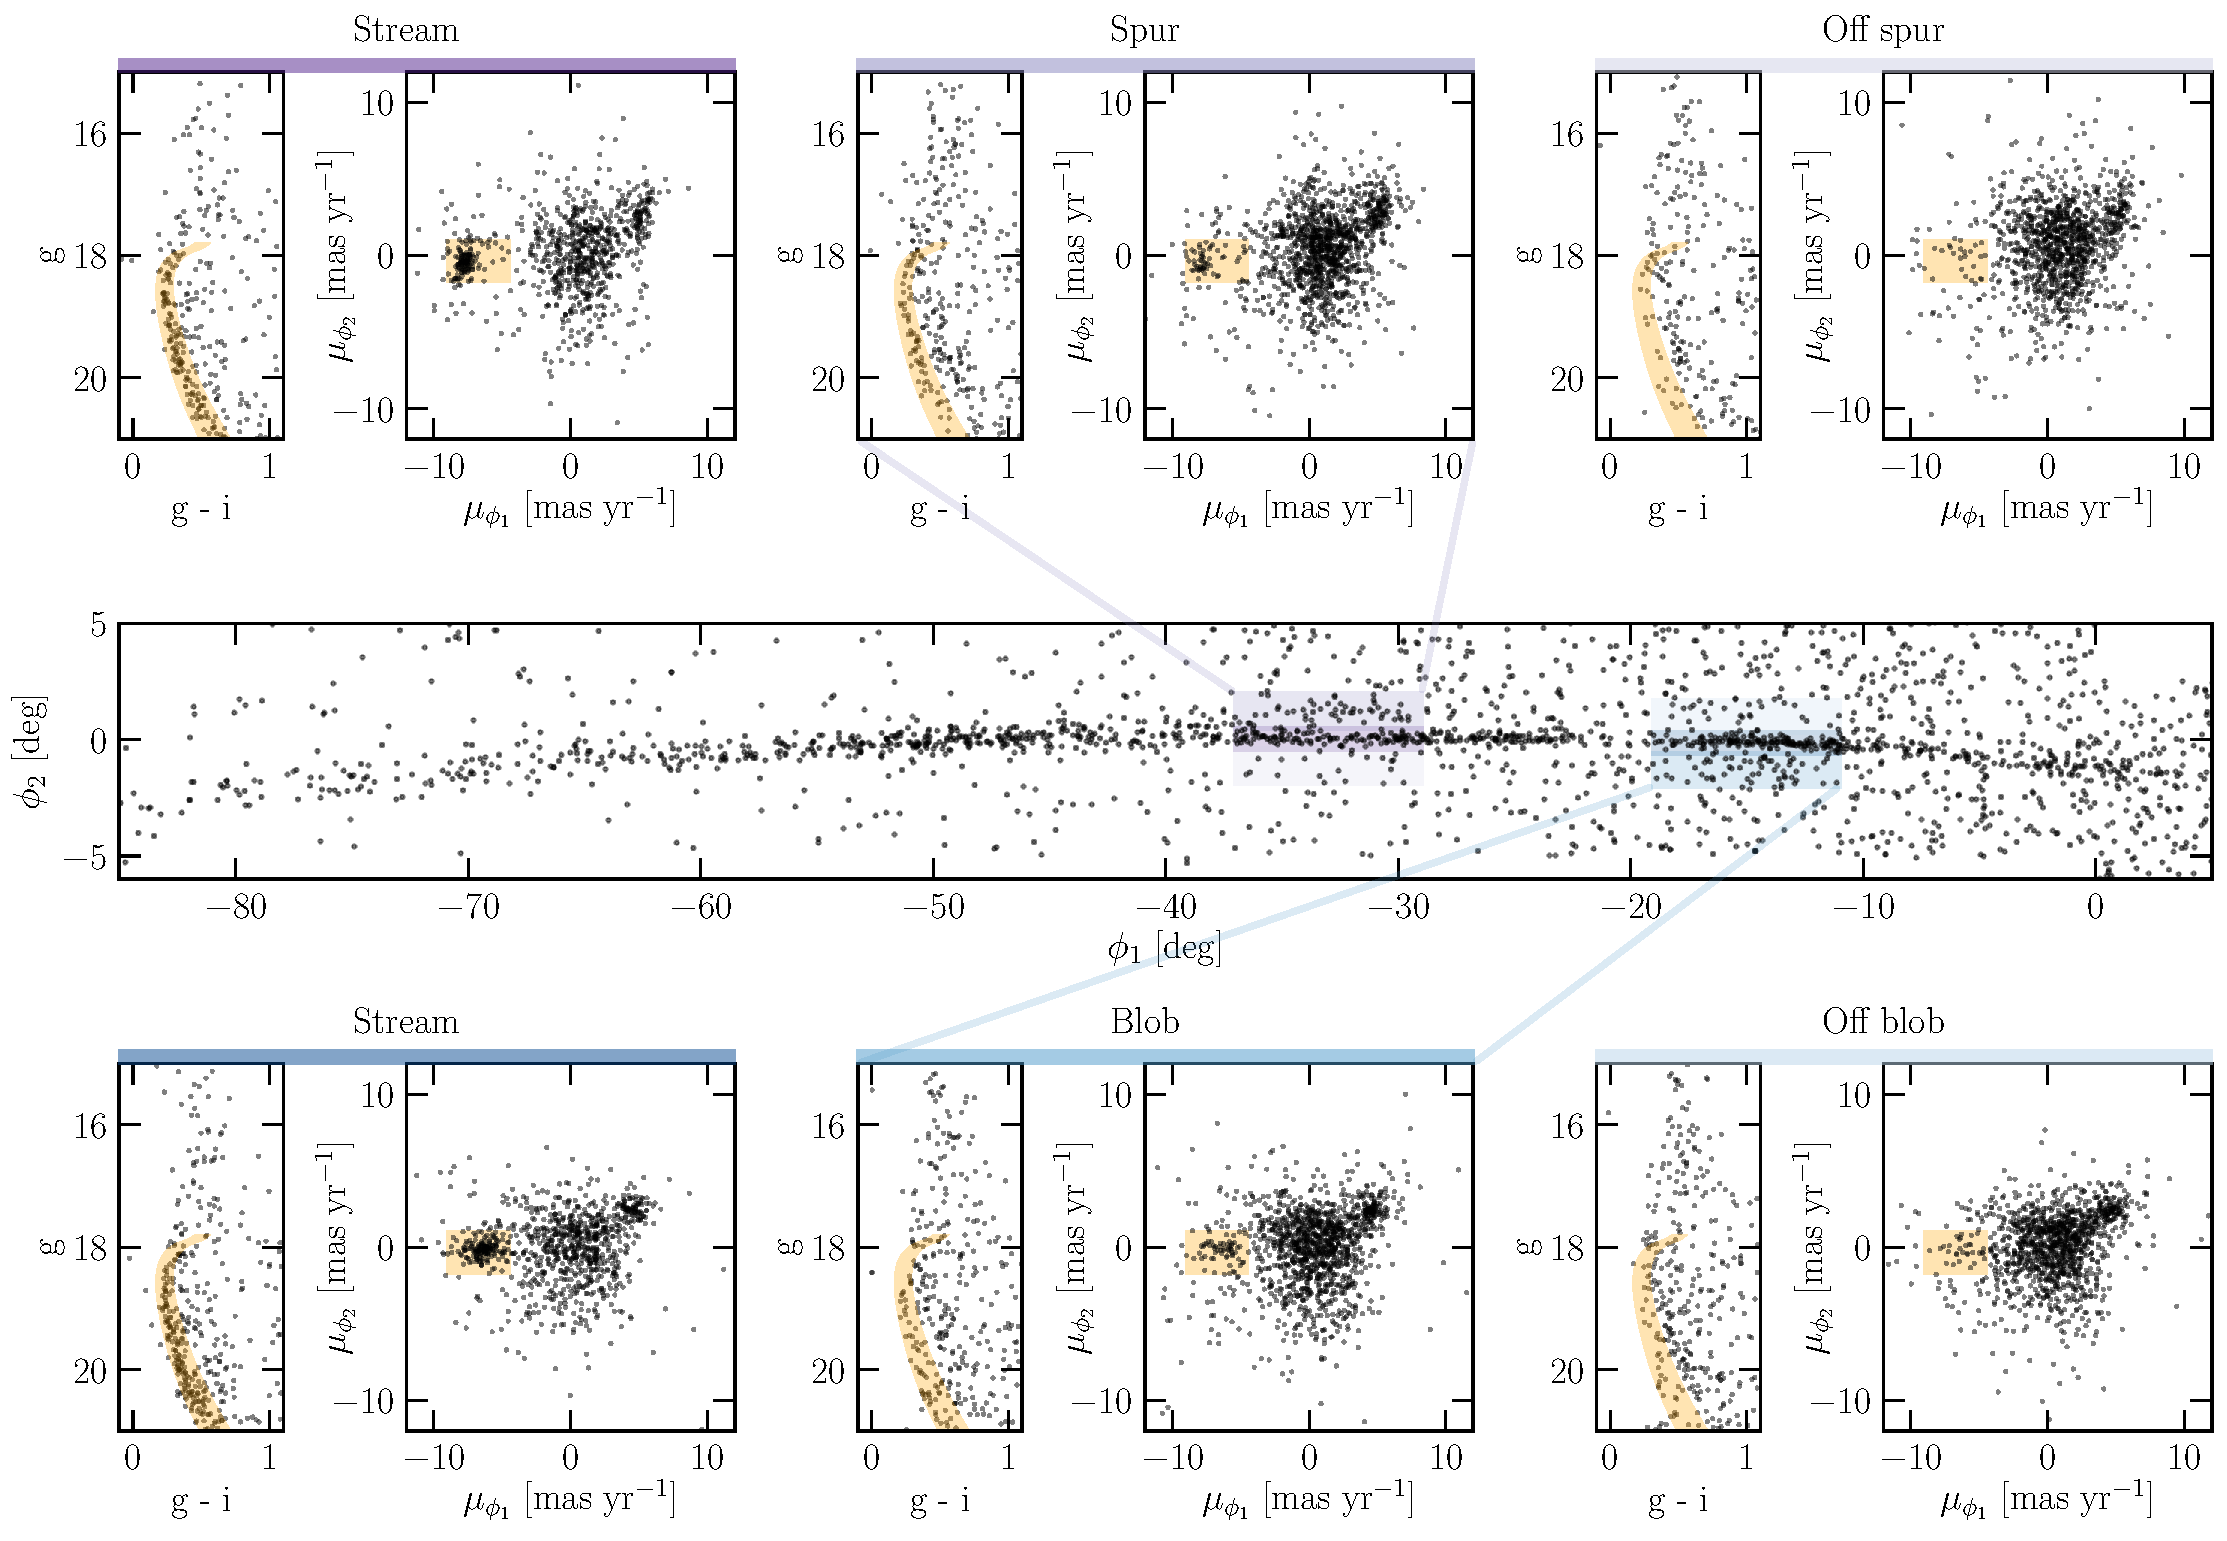
\includegraphics[width=\textwidth]{features.pdf}
\end{center}
\caption{%
\todo{AB}
\label{fig:features}
}
\end{figure}

\figurename~\ref{fig:features} (middle panel) again shows the proper-motion and CMD selected stream stars, with interesting features

\section{Discussion}
\label{sec:discussion}

\begin{figure}[h]
\begin{center}
% \includegraphics[width=\textwidth]{spur.pdf}
\end{center}
\caption{%
\todo{APW}
\label{fig:orbit}
}
\end{figure}

- novel way to identify members -- helpful that retrograde, but hopefully also applicable to other streams as kinematic important
- gd-1 even longer -- useful for potential constraints --> future

- progenitor? if confirmed, can create more realistic models (so far only modeled the whole stream as just a leading or trailing arm)
- to confirm -- measure actions, which change direction (some bovy paper)?

- no longer simple stream, discuss possible causes
- evaporation?

- smooth component of the potential?
-- show orbit
-- chaos?
-- bar?

- encounters?
-- work out mass / time combinations in impulse approximation
-- comment on GMC vs subhalo

- future:
-- radial velocities, measure 3d velocity structure (unique predictions)
-- tests for other outstanding issues
-- model facets of stream morphology to ascertain if consistent with encounter signatures


% \section{Conclusions}
% \label{sec:conclusions}

% From the combined proper motion and CMD selection of stream members
% (\sectionname~\ref{sec:data}), it is now clear that the GD-1 stream extends
% at least $90^\circ$ in apparent length.
% Several clear under-densities and gaps are also
% \figurename~\ref{fig:sfd-cmd} (middle panel) again shows the proper-motion and CMD selected stream stars, with several features


\acknowledgements{
It is a pleasure to thank
Vasily Belokurov,
Andrew R. Casey,
Marla Geha,
David W. Hogg,
Benjamin D. Johnson,
Kathryn V. Johnston,
Sergey Koposov,
Mariangela Lisanti,
Edward Schlafly,
and David N. Spergel for useful discussions and feedback.

This work has made use of data from the European Space Agency (ESA) mission {\it
Gaia} (\url{https://www.cosmos.esa.int/gaia}), processed by the {\it Gaia} Data
Processing and Analysis Consortium (DPAC,
\url{https://www.cosmos.esa.int/web/gaia/dpac/consortium}). Funding for the DPAC
has been provided by national institutions, in particular the institutions
participating in the {\it Gaia} Multilateral Agreement.  This research was
started at the NYC Gaia DR2 Workshop at the Center for Computational
Astrophysics of the Flatiron Institute in 2018 April.

AB acknowledges generous support from the Institute for Theory and Computation
at Harvard University.
All code used in this work and all results are available at
\url{https://github.com/adrn/GD1-DR2}.
}

\software{
    \package{Astropy} \citep{astropy},
    \package{dustmaps}\footnote{\url{https://github.com/gregreen/dustmaps}},
    \package{gala} \citep{gala},
    \package{IPython} \citep{ipython},
    \package{matplotlib} \citep{mpl},
    \package{numpy} \citep{numpy},
    \package{scipy} \citep{scipy}
}

\bibliographystyle{aasjournal}
\bibliography{gd1}

\clearpage

\appendix
\section{Completeness and the \gaia\ scanning pattern}
\label{sec:completeness}

% % Notebook:
% \begin{figure}[h]
% \begin{center}
% \includegraphics[width=0.7\textwidth]{nvisits.pdf}
% \end{center}
% \caption{%
% TODO
% \label{fig:TODO}
% }
% \end{figure}


\end{document}
